\documentclass[UTF8,fontset=none,12pt]{ctexart}

\setCJKmainfont{Songti SC}
\setCJKsansfont{PingFang SC}
\setCJKmonofont{Songti SC}

\usepackage[a4paper,margin=2.35cm]{geometry}
\usepackage{amsmath,amssymb,amsthm,mathtools,bm}
\usepackage{graphicx}
\usepackage{float}
\usepackage{booktabs}
\usepackage{enumitem}
\usepackage[hidelinks]{hyperref}

\newcommand{\C}{\mathbb{C}}
\newcommand{\R}{\mathbb{R}}
\newcommand{\range}{\operatorname{range}}
\newcommand{\rhoop}{\operatorname{\rho}}
\newcommand{\rank}{\operatorname{rank}}
\theoremstyle{definition}
\newtheorem{theorem}{定理}
\renewcommand{\thetheorem}{12.\arabic{theorem}}
\renewcommand{\thefigure}{12.\arabic{figure}}

\title{数值线性代数\quad 第 12 讲：良态性与条件数}
\author{Lloyd N. Trefethen、David Bau III\quad 中文阅读版}
\date{}

\begin{document}
\maketitle
\pagestyle{plain}

从本讲开始进入本书第三部分，系统讨论数值分析中两个此前只略有涉及的基本问题.\textbf{良态性（conditioning）}描述数学问题对扰动的反应；\textbf{稳定性（stability）}描述计算机上求解该问题的算法对扰动的反应.

\section*{问题的良态性}

抽象地看，可以把一个问题视为从数据所在的赋范向量空间 $X$ 到解所在的赋范向量空间 $Y$ 的函数
\[
    f:X\to Y.
\]
这个函数通常是非线性的（即使在线性代数中也是如此），但大多数时候至少是连续的.

我们通常关心问题 $f$ 在某个特定数据点 $x\in X$ 处的行为；这种行为可能随数据点而显著变化.把问题 $f$ 与规定的数据 $x$ 结合起来，可以称为一个\textbf{问题实例}，但通常也会直接把这个实例称为问题.

一个良态问题（实例）具有这样的性质：$x$ 的所有小扰动只会导致 $f(x)$ 的小变化.一个病态问题则具有这样的性质：某些很小的 $x$ 的扰动会导致 $f(x)$ 发生很大的变化.

这里“小”和“大”的含义取决于应用.有时，最合适的是用绝对尺度衡量扰动；有时，更合适的是相对于被扰动对象的范数来衡量.

\section*{绝对条件数}

设 $\delta x$ 表示 $x$ 的一个小扰动，并记
\[
    \delta f=f(x+\delta x)-f(x).
\]
问题 $f$ 在 $x$ 处的\textbf{绝对条件数} $\widehat\kappa=\widehat\kappa(x)$ 定义为
\begin{equation}
    \widehat\kappa
    =\lim_{\delta\to0}\ 
    \sup_{\|\delta x\|\le\delta}
    \frac{\|\delta f\|}{\|\delta x\|}.
    \tag{12.1}
\end{equation}
对大多数问题，这个上确界的极限可以理解为对所有无穷小扰动 $\delta x$ 取上确界.为便于阅读，下面通常直接写成
\begin{equation}
    \widehat\kappa=\sup_{\delta x}\frac{\|\delta f\|}{\|\delta x\|},
    \tag{12.2}
\end{equation}
并默认 $\delta x$ 和 $\delta f$ 是无穷小量.

如果 $f$ 可微，就可以通过 $f$ 的导数计算条件数.令 $J(x)$ 为矩阵，其第 $i,j$ 个元素是
\[
    \left.\frac{\partial f_i}{\partial x_j}\right|_x,
\]
它称为 $f$ 在 $x$ 处的 Jacobian.由导数定义，
\[
    \delta f\approx J(x)\delta x,
\]
且当 $\|\delta x\|\to0$ 时等式在极限意义下成立.于是绝对条件数为
\begin{equation}
    \widehat\kappa=\|J(x)\|,
    \tag{12.3}
\end{equation}
其中 $\|J(x)\|$ 表示由 $X,Y$ 上的范数诱导出的矩阵范数.

\section*{相对条件数}

如果关心的是相对变化，就需要相对条件的概念.问题 $f$ 在 $x$ 处的\textbf{相对条件数} $\kappa=\kappa(x)$ 定义为
\begin{equation}
    \kappa
    =\lim_{\delta\to0}\ 
    \sup_{\|\delta x\|\le\delta}
    \left(
    \frac{\|\delta f\|}{\|f(x)\|}
    \bigg/
    \frac{\|\delta x\|}{\|x\|}
    \right).
    \tag{12.4}
\end{equation}
同样，在默认 $\delta x$ 和 $\delta f$ 为无穷小量时，可以写成
\begin{equation}
    \kappa
    =\sup_{\delta x}
    \left(
    \frac{\|\delta f\|}{\|f(x)\|}
    \bigg/
    \frac{\|\delta x\|}{\|x\|}
    \right).
    \tag{12.5}
\end{equation}
如果 $f$ 可微，则
\begin{equation}
    \kappa=\frac{\|J(x)\|}{\|f(x)\|/\|x\|}.
    \tag{12.6}
\end{equation}

绝对和相对条件数都有用，但后者在数值分析中更重要.根本原因是计算机使用的浮点运算引入的通常是相对误差，而不是绝对误差；下一讲将讨论这一点.当 $\kappa$ 较小时（例如 $1,10,10^2$），问题称为良态；当 $\kappa$ 很大时（例如 $10^6,10^{16}$），问题称为病态.

\section*{例子}

\subsection*{例 12.1}

考虑从 $x\in\C$ 计算标量 $x/2$ 这一平凡问题.函数 $f:x\mapsto x/2$ 的 Jacobian 就是导数 $J=f'=1/2$.由式 (12.6)，
\[
    \kappa
    =\frac{\|J\|}{\|f(x)\|/\|x\|}
    =\frac{1/2}{(x/2)/x}
    =1.
\]
按任何通常标准，这都是良态问题.

\subsection*{例 12.2}

考虑在 $x>0$ 时计算 $\sqrt{x}$ 的问题.函数 $f:x\mapsto\sqrt{x}$ 的 Jacobian 为
\[
    J=f'=\frac{1}{2\sqrt{x}}.
\]
因此
\[
    \kappa
    =\frac{\|J\|}{\|f(x)\|/\|x\|}
    =\frac{1/(2\sqrt{x})}{\sqrt{x}/x}
    =\frac12.
\]
这同样是良态问题.

\subsection*{例 12.3}

考虑从向量 $x=(x_1,x_2)^*\in\C^2$ 计算标量
\[
    f(x)=x_1-x_2
\]
的问题.为简单起见，在数据空间 $\C^2$ 上使用 $\infty$-范数. $f$ 的 Jacobian 是
\[
    J=
    \begin{bmatrix}
        \dfrac{\partial f}{\partial x_1}&
        \dfrac{\partial f}{\partial x_2}
    \end{bmatrix}
    =
    \begin{bmatrix}1&-1\end{bmatrix},
    \qquad \|J\|_\infty=2.
\]
所以条件数为
\[
    \kappa
    =\frac{\|J\|_\infty}{\|f(x)\|/\|x\|_\infty}
    =
    \frac{2}{|x_1-x_2|/\max\{|x_1|,|x_2|\}}.
\]
当 $|x_1-x_2|\approx0$ 时，这个量很大.因此，当 $x_1\approx x_2$ 时问题是病态的，这与我们对“消去误差”危险性的直觉一致.

\subsection*{例 12.4}

考虑在 $x$ 接近 $10^{100}$ 时计算 $f(x)=\tan x$.在这个问题中，$x$ 的极小相对扰动也可能导致 $\tan x$ 发生任意大的变化.结果是：在大多数计算机上，$\tan(10^{100})$ 实际上不可计算.同样的微小扰动也会导致 $\tan x$ 的导数发生任意变化，因此除了观察到导数并不小之外，试图计算 Jacobian 没有多大意义.想了解一个结局依赖于 $\tan(10^{100})$ 这种病态性的故事，可以参阅 Richard Feynman 的《别闹了，费曼先生》中的 “Lucky Numbers”.

\subsection*{例 12.5}

给定多项式系数后求根，是病态问题的经典例子.考虑
\[
    x^2-2x+1=(x-1)^2,
\]
它在 $x=1$ 处有一个二重根.系数的一个小扰动可能导致根发生更大的变化；例如
\[
    x^2-2x+0.9999=(x-0.99)(x-1.01).
\]
事实上，在这里根的变化量可以与系数变化量的平方根成正比.因此 Jacobian 是无穷大（问题不可微），并且 $\kappa=\infty$.

即使不涉及多重根，多项式求根通常也很病态.如果多项式 $p(x)$ 的第 $i$ 个系数 $a_i$ 受到无穷小扰动 $\delta a_i$，第 $j$ 个根 $x_j$ 的扰动满足一阶关系
\[
    \delta x_j\approx-\frac{\delta a_i\,x_j^i}{p'(x_j)},
\]
其中 $p'$ 表示 $p$ 的导数.因此，相对于单个系数 $a_i$ 的扰动，根 $x_j$ 的条件数为
\begin{equation}
    \kappa
    =
    \frac{|\delta x_j|/|x_j|}{|\delta a_i|/|a_i|}
    \approx
    \frac{|a_i x_j^{i-1}|}{|p'(x_j)|}.
    \tag{12.7}
\end{equation}
这个数往往非常大.考虑“Wilkinson 多项式”
\begin{equation}
    p(x)=\prod_{i=1}^{20}(x-i)
    =a_0+a_1x+\cdots+a_{19}x^{19}+x^{20}.
    \tag{12.8}
\end{equation}
这个多项式最敏感的根是 $x=15$，它对系数 $a_{15}\approx1.67\times10^9$ 的变化最敏感.相应的条件数为
\[
    \kappa
    \approx
    \frac{1.67\times10^9\cdot15^{14}}{5!\,14!}
    \approx5.1\times10^{13}.
\]
图~\ref{fig:12-1} 从图形上展示了这种病态性.

\begin{figure}[H]
    \centering
    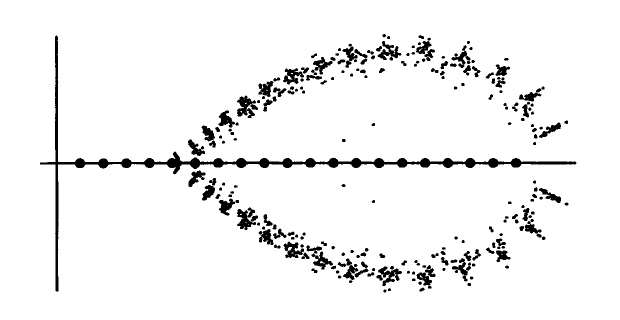
\includegraphics[width=0.80\linewidth]{../assets/figure-12-1.png}
    \caption{Wilkinson 多项式的经典病态性例子.大黑点是未扰动多项式 (12.8) 的根；小点是 100 个随机扰动多项式在复平面中的根叠加图.扰动系数为 $\widetilde a_k=a_k(1+10^{-10}r_k)$，其中 $r_k$ 来自均值为 0、方差为 1 的正态分布.}
    \label{fig:12-1}
\end{figure}

\subsection*{例 12.6}

计算非对称矩阵的特征值也常常是病态的.比较下面两个矩阵：
\[
    \begin{bmatrix}1&1000\\0&1\end{bmatrix},
    \qquad
    \begin{bmatrix}1&1000\\0.001&1\end{bmatrix}.
\]
它们的特征值分别是 $\{1,1\}$ 和 $\{0,2\}$.另一方面，如果矩阵 $A$ 是对称的（更一般地，如果 $A$ 是正规矩阵），那么它的特征值是良态的.可以证明：若 $\lambda$ 与 $\lambda+\delta\lambda$ 分别是 $A$ 与 $A+\delta A$ 的对应特征值，则
\[
    |\delta\lambda|\le\|\delta A\|_2,
\]
当 $\delta A$ 是单位矩阵的倍数时取等号（见习题 26.3）.因此，用 2-范数衡量扰动时，对称特征值问题的绝对条件数是 $\widehat\kappa=1$，相对条件数为
\[
    \kappa=\frac{\|A\|_2}{|\lambda|}.
\]

\section*{矩阵--向量乘法的条件}

现在讨论数值线性代数中一个极其重要的条件数.固定 $A\in\C^{m\times n}$，考虑从输入 $x$ 计算 $Ax$ 的问题；也就是说，只扰动 $x$ 而不扰动 $A$，并求相应的条件数.设 $\|\cdot\|$ 是任意向量范数，矩阵范数取相应的诱导范数.直接从 $\kappa$ 的定义出发，可得
\[
\begin{aligned}
\kappa
&=\sup_{\delta x}
\left(
\frac{\|A(x+\delta x)-Ax\|}{\|Ax\|}
\bigg/
\frac{\|\delta x\|}{\|x\|}
\right)\\
&=\sup_{\delta x}
\frac{\|A\delta x\|}{\|\delta x\|}
\bigg/
\frac{\|Ax\|}{\|x\|}.
\end{aligned}
\]
因此
\begin{equation}
    \kappa=\|A\|\frac{\|x\|}{\|Ax\|}.
    \tag{12.9}
\end{equation}
这是式 (12.6) 的一个特殊情形，也是一个同时依赖于 $A$ 和 $x$ 的精确公式.

假设 $A$ 恰好是方阵且非奇异.由于
\[
    \frac{\|x\|}{\|Ax\|}\le\|A^{-1}\|,
\]
式 (12.9) 可放宽为与 $x$ 无关的界：
\begin{equation}
    \kappa\le\|A\|\|A^{-1}\|.
    \tag{12.10}
\end{equation}
也可以写成
\begin{equation}
    \kappa=\alpha\|A\|\|A^{-1}\|,
    \tag{12.11}
\end{equation}
其中
\begin{equation}
    \alpha=
    \frac{\|x\|/\|Ax\|}{\|A^{-1}\|}.
    \tag{12.12}
\end{equation}
对某些 $x$，有 $\alpha=1$，从而 $\kappa=\|A\|\|A^{-1}\|$.如果使用 2-范数，当 $x$ 是 $A$ 的最小右奇异向量的倍数时就会发生这种情况.

事实上，$A$ 不必是方阵.如果 $A\in\C^{m\times n}$、$m\ge n$ 且满列秩，那么式 (12.10)--(12.12) 仍成立，只需把 $A^{-1}$ 换成第 11 讲定义的伪逆 $A^+$.

那么逆问题如何处理：给定 $A$，从输入 $b$ 计算 $A^{-1}b$？从数学上说，这与刚才的问题完全相同，只是把其中的 $A$ 换成了 $A^{-1}$.于是可以得到下面的定理.

\begin{theorem}
设 $A\in\C^{m\times m}$ 非奇异，并考虑方程 $Ax=b$.相对于 $x$ 的扰动，从 $x$ 计算 $b$ 的问题的条件数为
\begin{equation}
    \kappa=\|A\|\frac{\|x\|}{\|b\|}
    \le\|A\|\|A^{-1}\|.
    \tag{12.13}
\end{equation}
相对于 $b$ 的扰动，从 $b$ 计算 $x$ 的问题的条件数为
\begin{equation}
    \kappa=\|A^{-1}\|\frac{\|b\|}{\|x\|}
    \le\|A\|\|A^{-1}\|.
    \tag{12.14}
\end{equation}
如果 $\|\cdot\|=\|\cdot\|_2$，那么在式 (12.13) 中，当 $x$ 是对应于最小奇异值 $\sigma_m$ 的右奇异向量的倍数时取等号；在式 (12.14) 中，当 $b$ 是对应于最大奇异值 $\sigma_1$ 的左奇异向量的倍数时取等号.
\end{theorem}

\section*{矩阵的条件数}

乘积
\[
    \|A\|\|A^{-1}\|
\]
出现得如此频繁，以至于它有了自己的名字：矩阵 $A$（相对于范数 $\|\cdot\|$）的\textbf{条件数}，记为
\begin{equation}
    \kappa(A)=\|A\|\|A^{-1}\|.
    \tag{12.15}
\end{equation}
此时，“条件数”一词指的是矩阵，而不是某个具体问题.如果 $\kappa(A)$ 小，称 $A$ 良态；如果 $\kappa(A)$ 大，称 $A$ 病态.如果 $A$ 奇异，通常约定 $\kappa(A)=\infty$.

注意，如果 $\|\cdot\|=\|\cdot\|_2$，则
\[
    \|A\|_2=\sigma_1,\qquad \|A^{-1}\|_2=\frac1{\sigma_m}.
\]
因此在 2-范数下
\begin{equation}
    \kappa(A)=\frac{\sigma_1}{\sigma_m}.
    \tag{12.16}
\end{equation}
这正是计算矩阵 2-范数条件数时通常使用的公式.对于 $A$ 的单位球，线性映像是一个超椭球，$\sigma_1/\sigma_m$ 可以理解为它的偏心程度（图 4.1）.

对于满列秩的长方形矩阵 $A\in\C^{m\times n}$、$m\ge n$，条件数用伪逆定义：
\[
    \kappa(A)=\|A\|\|A^+\|.
\]
由于伪逆的定义源于最小二乘问题，这个定义在 $\|\cdot\|=\|\cdot\|_2$ 时最有用，此时
\begin{equation}
    \kappa(A)=\frac{\sigma_1}{\sigma_n}.
    \tag{12.17}
\end{equation}

\section*{方程组的条件}

在定理 12.1 中，我们固定 $A$，扰动 $x$ 或 $b$.如果扰动 $A$，情况会怎样？具体地，固定 $b$，考虑问题
\[
    A\mapsto x=A^{-1}b
\]
在 $A$ 受到无穷小扰动 $\delta A$ 时的行为.此时 $x$ 必须发生无穷小变化 $\delta x$，并满足
\[
    (A+\delta A)(x+\delta x)=b.
\]
利用 $Ax=b$，并舍去二阶无穷小项 $(\delta A)(\delta x)$，得到
\[
    (\delta A)x+A(\delta x)=0,
    \qquad
    \delta x=-A^{-1}(\delta A)x.
\]
因此
\[
    \|\delta x\|\le\|A^{-1}\|\|\delta A\|\|x\|,
\]
或者等价地，
\[
    \frac{\|\delta x\|/\|x\|}{\|\delta A\|/\|A\|}
    \le\|A^{-1}\|\|A\|=\kappa(A).
\]
当 $\delta A$ 满足
\[
    \|A^{-1}(\delta A)x\|
    =\|A^{-1}\|\|\delta A\|\|x\|
\]
时，这个界取等号.利用对偶范数（习题 3.6）可以证明，对任意 $A,b$ 和范数 $\|\cdot\|$，都存在这样的扰动 $\delta A$.于是得到下面的结果.

\begin{theorem}
设 $b$ 固定，考虑计算 $x=A^{-1}b$ 的问题，其中 $A$ 是方阵且非奇异.相对于 $A$ 的扰动，该问题的条件数为
\begin{equation}
    \kappa=\|A\|\|A^{-1}\|=\kappa(A).
    \tag{12.18}
\end{equation}
\end{theorem}

定理 12.1 和定理 12.2 对数值线性代数极其重要，因为它们决定了解线性方程组时可能达到的准确度.如果一个方程组 $Ax=b$ 包含病态矩阵 $A$，除非有非常特殊的情况，否则计算解时总应预期“损失 $\log_{10}\kappa(A)$ 位数字”.后面还会回到这一现象；第 18 讲将讨论最小二乘问题的类似结果.

\section*{习题}

\begin{enumerate}[label=\textbf{12.\arabic*}]
    \item 设 $A$ 是一个 $202\times202$ 矩阵，满足 $\|A\|_2=100$ 且 $\|A\|_F=101$.给出矩阵 2-范数条件数 $\kappa(A)$ 的最精确可能下界.

    \item 第 11 讲例 11.1 提到，等距点上的多项式插值是病态的.为了说明这一现象，设 $x_1,\ldots,x_n$ 和 $y_1,\ldots,y_m$ 分别是从 $-1$ 到 1 的 $n$ 个、$m$ 个等距点.
    \begin{enumerate}[label=(\alph*)]
        \item 推导一个 $m\times n$ 矩阵 $A$ 的公式，使它把在 $\{x_i\}$ 上给定的 $n$ 维数据向量映射为采样值 $\{p(y_j)\}$ 组成的 $m$ 维向量，其中 $p$ 是这些数据的 $n-1$ 次多项式插值（见例 1.1）.
        \item 编写程序，在 $n=1,2,\ldots,30$、$m=2n-1$ 时计算 $A$，并在半对数坐标下绘制 $\|A\|_\infty$.当 $m\to\infty$ 时，$\|A\|_\infty$ 的连续极限称为等距插值的 Lebesgue 常数；当 $n\to\infty$ 时，它渐近于
        \[
            \frac{2^n}{e(n-1)\log n}.
        \]
        \item 对 $n=1,2,\ldots,30$、$m=2n-1$，插值常数函数 1 的问题的 $\infty$-范数条件数 $\kappa$ 是多少？使用式 (12.6).
        \item 当 $n=11$ 时，你的结果与图 11.1 所隐含的界有多接近？
    \end{enumerate}

    \item 本题的目标是探索随机矩阵的一些性质.你的任务是像实验室科学家一样进行实验，从实验中提出猜想，再设计更细致的实验.不要尝试证明任何结论，但要制作精心设计的图；一幅好图胜过千言万语.

    定义随机矩阵为 $m\times m$ 矩阵，其元素是独立同分布的实正态随机变量，均值为 0、标准差为 $m^{-1/2}$.在 MATLAB 中可写为
    \[
        A=\operatorname{randn}(m,m)/\sqrt m.
    \]
    引入因子 $\sqrt m$ 是为了使 $m\to\infty$ 时的极限行为更整洁.
    \begin{enumerate}[label=(\alph*)]
        \item 随机矩阵的特征值看起来是什么样？如果取 100 个随机矩阵，把它们的全部特征值叠加在一张图上，会发生什么？当 $m=8,16,32,64,\ldots$ 时进行这项实验，会暗示什么模式？当 $m\to\infty$ 时，谱半径 $\rho(A)$ 如何变化（见习题 3.2）？
        \item 范数会怎样？当 $m\to\infty$ 时，随机矩阵的 2-范数如何变化？当然必须有 $\rho(A)\le\|A\|$（习题 3.2）.当 $m\to\infty$ 时，这个不等式看起来是否趋于等式？
        \item 条件数，或者更简单地说，最小奇异值 $\sigma_{\min}$ 如何变化？即使固定 $m$，这个问题也很有趣.在 $\mathbb R^{m\times m}$ 的随机矩阵中，似乎有多大比例满足 $\sigma_{\min}\le2^{-1},4^{-1},8^{-1},\ldots$？换言之，最小奇异值概率分布的尾部是什么样？当 $m$ 变化时，这一切的尺度如何变化？
        \item 如果考虑随机三角矩阵而不是完整矩阵，即元素来自同一分布的上三角矩阵，(a)--(c) 的答案如何变化？
    \end{enumerate}
\end{enumerate}

\end{document}
